%Positionering
\subsubsection{Software}
Programmet for \textbf{Positionscontrolleren} er designet på baggrund af systemarkitekturen samt de overvejelser, der er gjort i sektion \ref{pos_hw}. Det er \textbf{Positionscontrollerens} opgave at vurdere, om en vinflaske er indsat i WinePrep, og i så fald, om denne er kompatibel med systemet. Den skal da positionere \textbf{Åbningsmekanismen} således, at denne låser flasken i en fast position. \textbf{Positionscontrolleren} fungerer herved også som bindeled mellem \textbf{Brugergrænsefladen}, som den modtager kommandoer fra og giver meddelelser om flaskens status tilbage til, og \textbf{Åbningscontrolleren}. \\
\\
Ovennævnte grænseflader, samt de i sektion \ref{sub:Pos} nævnte motorer og sensorer, kan omsættes til 5 grænsefladeklasser: \\
\\
\textbf{DevKit\_SPI}, hvorigennem kommunikationen med \textbf{Brugergrænsefladen} foregår. \\
\textbf{PSoC\_SPI}, hvorigennem kommunikationen med \textbf{Åbningscontrolleren} foregår. \\
\textbf{MotorsXY}, som styrer motorerne for x- og y-akserne, hvis funktionalitet er identisk. \\
\textbf{MotorZ}, som styrer motorerne for z-aksen. \\
\textbf{Sensors}, som styrer sensorerne. \\

\myparagraph{Sekvensdiagram}
Sekvensdiagrammet i figur \ref{sd:Pos} viser, hvordan der kommunikeres mellem klasserne, og hvilken funktionalitet, disse indeholder.

\begin{figure}[H]
	\centerline{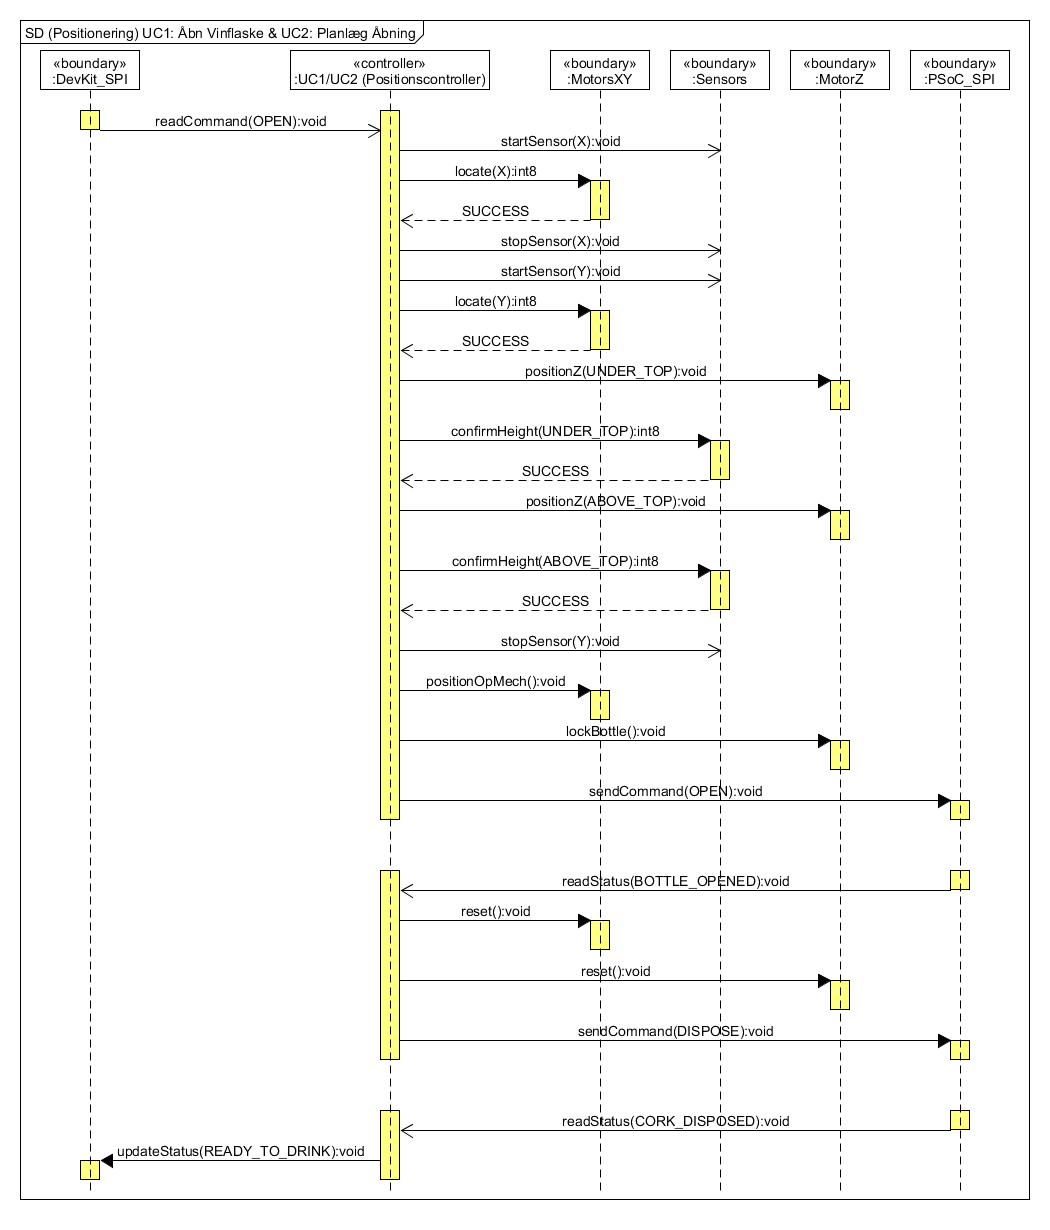
\includegraphics[scale=0.33]{tex/Design/PSoC/Diagrammer/SD_Positionering}}
	\caption{Sekvensdiagram over \textbf{Positionering}}
	\label{sd:Pos}
\end{figure}

\noindent Detektering og åbning af vinflasken påbegyndes ved en kommando fra \textbf{Brugergrænsefladen} til \textbf{Positionscontrolleren}, som efter at have fastslået flaskens x- og y-position checker at flasken har en korrekt højde ved først at løfte sensorerne til en position, der er en vis afstand under flaskens top og få bekræftet, at flasken kan detekteres, og derefter løfte sensorerne til en vis afstand over flaskens top og få bekræftet, at flasken ikke længere kan detekteres. Herefter flyttes åbningsmekanismen til en position over flasken, hvorefter denne fastlåses. Der gives da besked til \textbf{Åbningscontrolleren} om at åbne flasken. Efter dette er gjort indstiller \textbf{Positionscontrolleren} \textbf{Åbningsmekanismen} til dennes starposition, hvorefter der gives besked til \textbf{Åbningscontrolleren} om at dispensere proppen. Når dette er gjort gives der besked til \textbf{Brugergrænsefladen} om, at flasken er drikkeklar. \\
\\
Noget, som ikke er vist i sekvensdiagrammet, er fejlscenarier. Disse findes for de metoder, hvor der i diagrammet returneres \textit{SUCCESS}. I disse tilfælde resettes motorerne, og \textbf{Positionscontrolleren} sender en statusbesked til \textbf{Brugergrænsefladen} om den pågældende fejl.

\myparagraph{Funktionsbeskrivelse}
Programmets overordnede funktionalitet er ikke videre kompliceret, dog kan der for især locate(X)/locate(Y) findes grund til nærmere beskrivelse.
\\
\\
\textbf{locate(AXIS)} \\
For nærmere at beskrive denne metode er følgende aktivitetsdiagram blevet udarbejdet: \\

\begin{figure}[H]
	\centerline{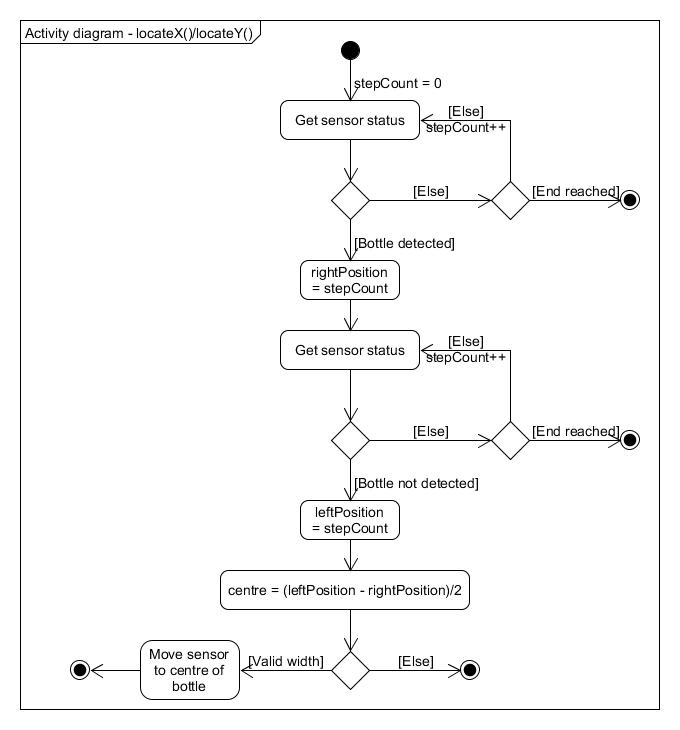
\includegraphics[scale=0.5]{tex/Design/PSoC/AD_locate.jpg}}
	\caption{Aktivitetsdiagram over locateX()/locateY()}
	\label{AD_locate}
\end{figure}

Ved indtrædelse i metoden nulstilles en tæller \textit{stepCount}, som tæller antallet af steps taget. Derefter måles med sensor, om en flaske er registreret. Så længe dette ikke er tilfældet, skal motoren fortsat køre, og \textit{stepCount} skal tælles op. I så fald enden på aksen nås, skal metoden afslutte og returnere en fejlværdi. Hvis flasken registreres, gemmes \textit{stepCount} i \textit{rightPosition}. Der fortsættes efter samme mønster, indtil der ikke længere registreres en flaske, eller enden er nået. Hvis førstnævnte er tilfældet, gemmes \textit{stepCount} i \textit{leftPosition}, hvorefter afstanden til flaskens midte beregnes ud fra \textit{rightPosition} og \textit{leftPosition}. Denne værdi sammenlignes med en forudbestemt værdi for at sikre, at det er en kompatibel flaske, der er indsat. Hvis ikke, afsluttes metoden og returnerer en fejlværdi. Ellers flyttes sensoren til flaskens midte, og metoden returnerer en succesværdi.
\\
\\
\textbf{Øvrige metoder}

\textbf{positionZ(POSITION)} løfter sensorerne et vist antal steps, som er bestemt ud fra det medgivne argument, op fra startpositionen.

\textbf{confirmHeight(POSITION)} skal registrere med y-sensoren om en flaske kan registreres i den givne højde alt efter den medgivne parameter (UNDER\_TOP: flaske skal registreres, ABOVE\_TOP: flaske skal ej registreres).

\textbf{positionXY()} skal ud fra forudbestemte værdier køre motorerne et vis antal steps mod åbningsmekanismens centrum.

\textbf{reset()} kører motorerne indtil deres respektive trykknap ved startpositionen er påtrykt.